\addtocontents{toc}{\protect\setcounter{tocdepth}{1}}
\chapter[Definición de la Empresa o Institución]{Definición de la Empresa o Institución}

\section[Descripción de la Empresa]{Descripción de la empresa}

\subsection*{Antecedentes generales}

El proyecto se desarrolla para el Complejo Asistencial Dr.~Sótero del Río, un
hospital público, asistencial y docente de alta complejidad ubicado en Avenida
Concha y Toro~3459, Puente Alto, Región Metropolitana \citep{hospital_sotero_2026}.
Su rubro es la atención de salud especializada, que abarca el diagnóstico, el
tratamiento, el seguimiento y la educación de pacientes. Entre ellos se
encuentran niños, niñas y adolescentes con cáncer que se atienden en su unidad de
oncología pediátrica, adscrita al Programa Infantil Nacional de Drogas
Antineoplásicas (PINDA) \citep{pinda_centros_2026}.

\subsection*{Entorno}

El hospital pertenece a la red pública del Servicio de Salud Metropolitano Sur
Oriente. Al tratarse de una institución pública, no compite por participación de
mercado. Coordina su labor con el Ministerio de Salud, con otros centros PINDA y
con organizaciones de apoyo al cáncer infantil, como la Fundación Nuestros Hijos
\citep{fundacion_nuestros_hijos_2026}. Su relevancia se mide por la cobertura que
entrega a la población del sector suroriente de Santiago y por la continuidad de
la atención entre el hospital y el hogar.

\subsection*{Misión, visión y objetivos}

La misión del hospital es \emph{``ser un hospital público asistencial docente de
alta complejidad que entrega atención humanizada, segura y de excelencia,
centrada en las personas y su bienestar biopsicosocial, mediante equipos
interdisciplinarios comprometidos con la calidad, equidad, innovación,
investigación y trabajo en red''}. Su visión es \emph{``ser un hospital de alta
complejidad, reconocido a nivel nacional e internacional por su atención
humanizada, excelencia clínica, innovación, docencia y liderazgo en
investigación''}.

Para este proyecto, los objetivos institucionales se traducen en fortalecer el
seguimiento del paciente oncológico pediátrico, apoyar al cuidador principal en
el manejo domiciliario y dar continuidad a la atención entre el hospital y el
hogar.

\subsection*{Estructura organizativa}

La Dirección encabeza la organización y de ella dependen seis subdirecciones:
Médica, de Gestión del Cuidado, de Gestión Administrativa, de Unidades de Apoyo,
de Gestión y Desarrollo de Personas y de Puesta en Marcha. La
Figura~\ref{fig:organigrama} muestra la estructura general.

\begin{figure}[H]
    \centering
    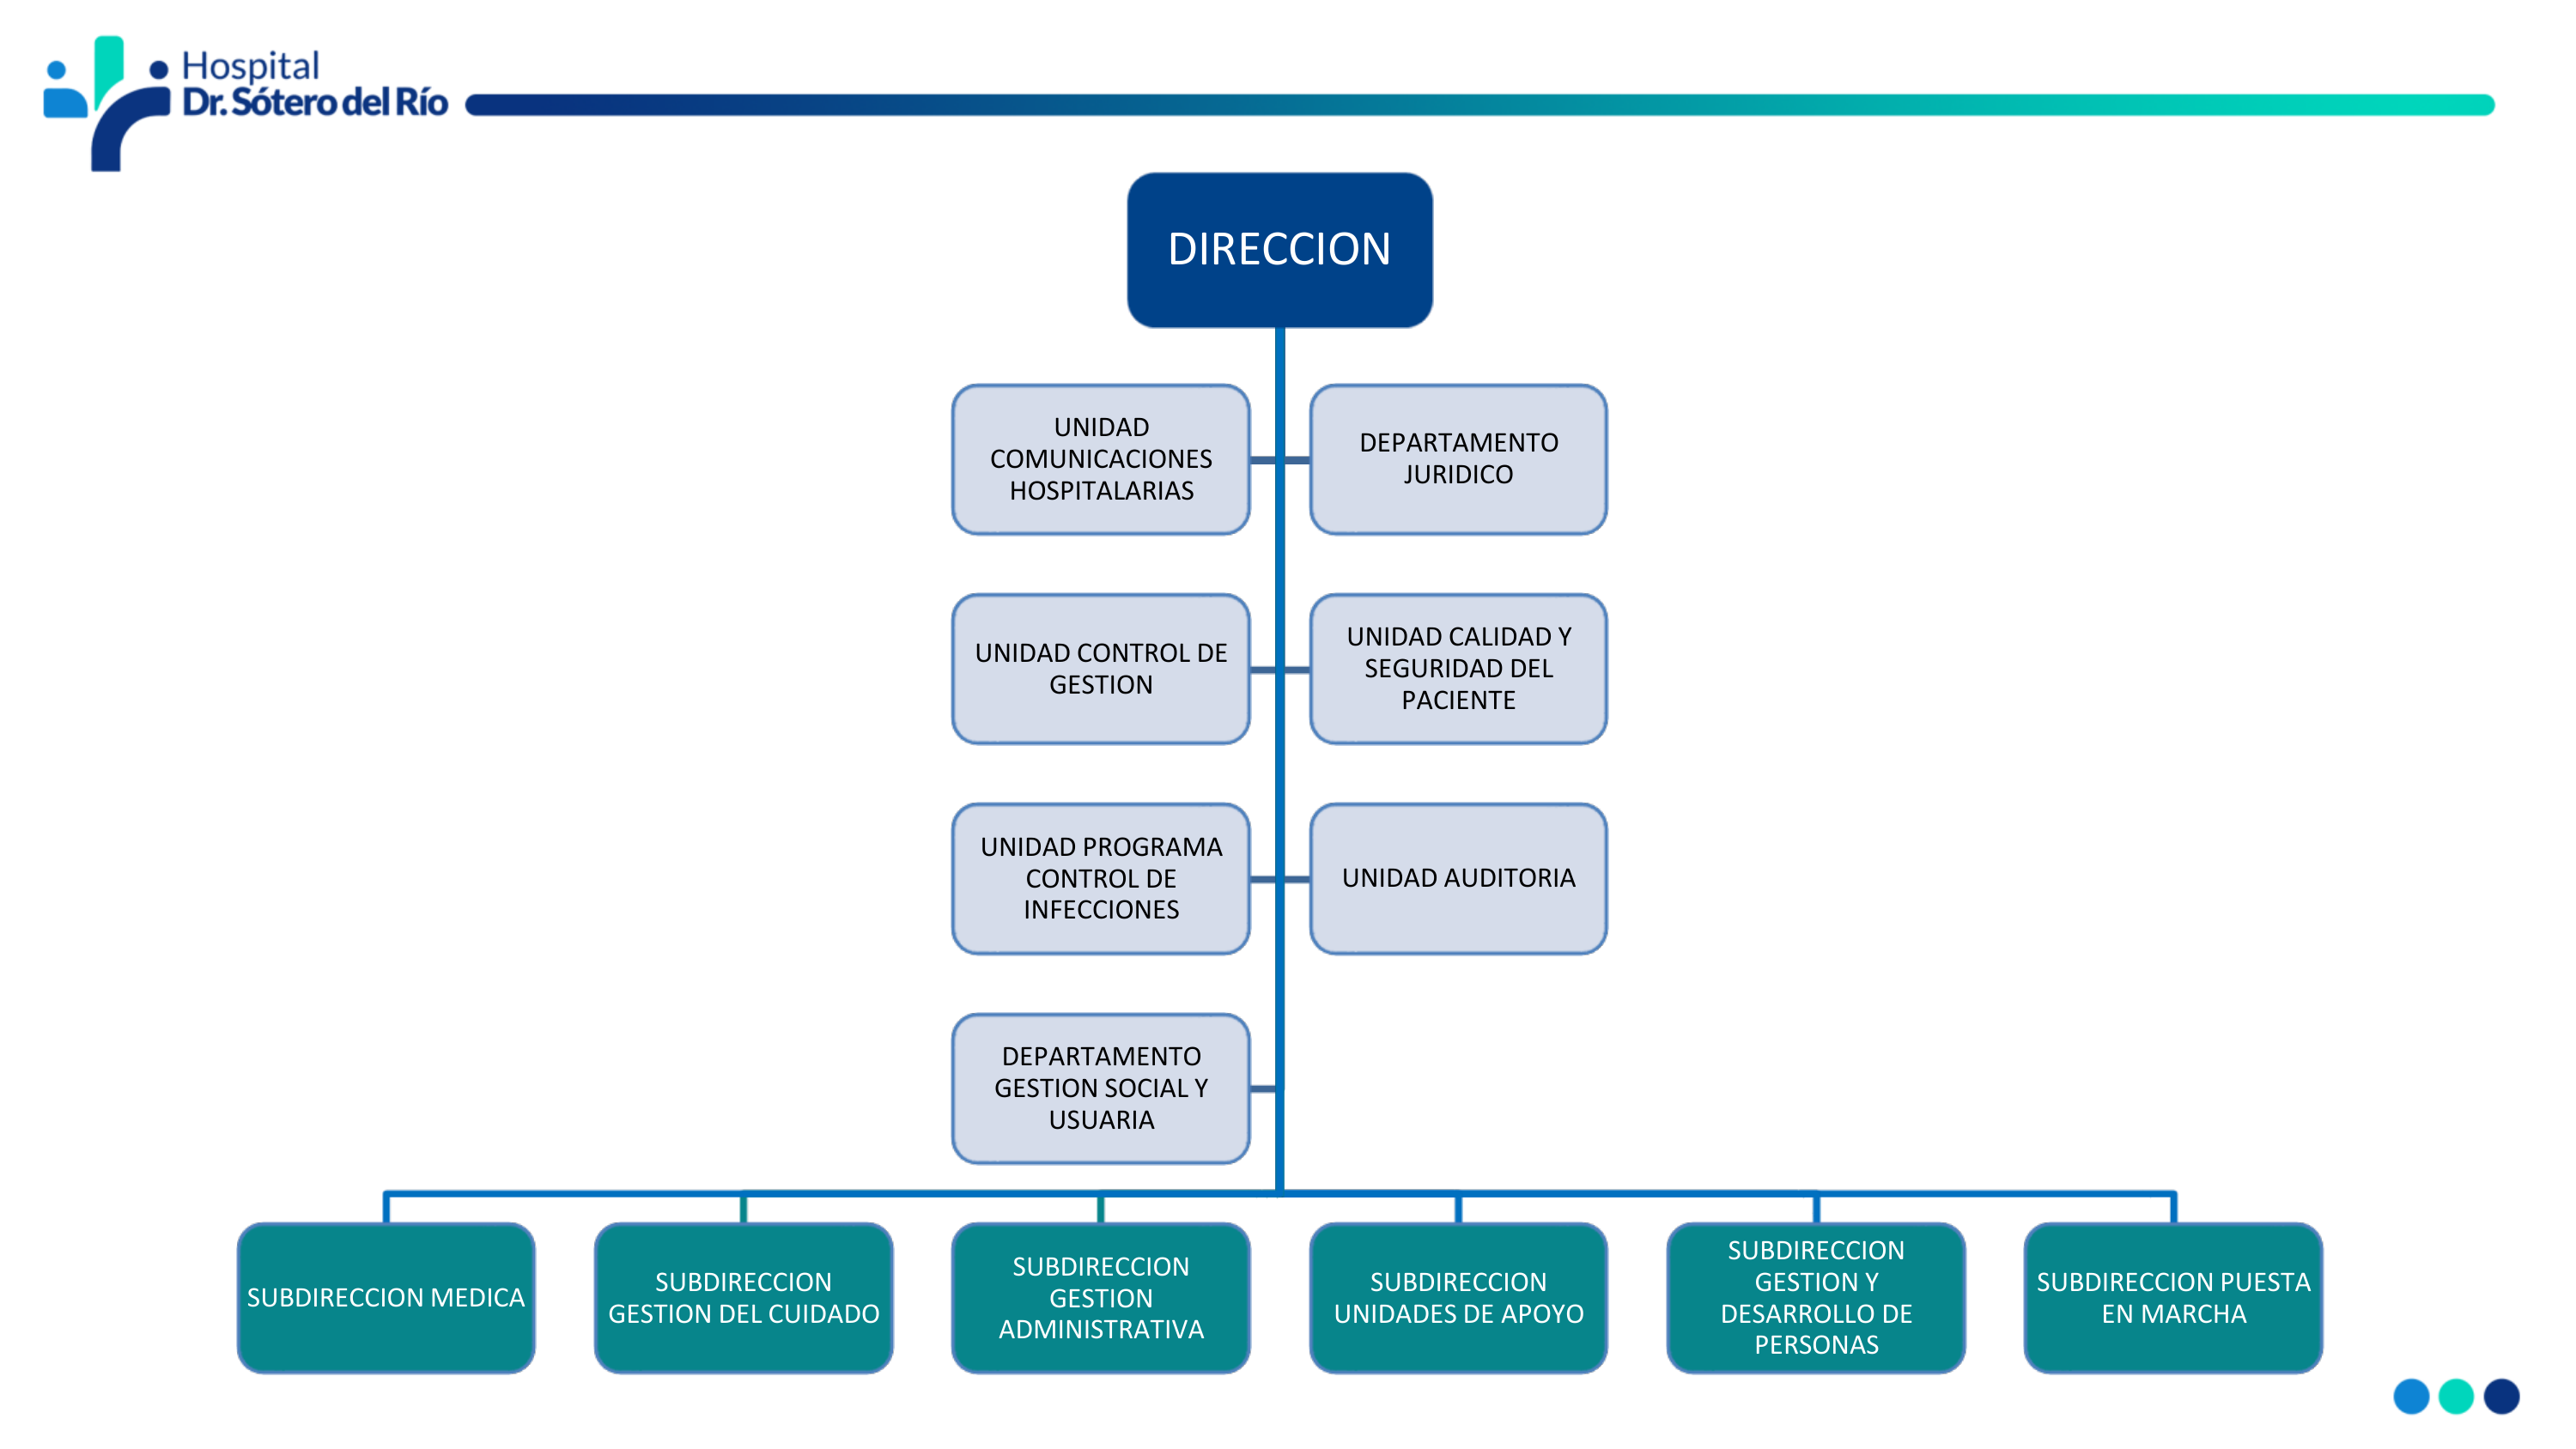
\includegraphics[width=\textwidth]{figures/organigrama_hsr-01.png}
    \caption{Organigrama del Complejo Asistencial Dr.~Sótero del Río.}
    \label{fig:organigrama}
\end{figure}

Para el proyecto resultan relevantes las funciones del equipo clínico de
oncología pediátrica. Este equipo entrega al cuidador las indicaciones de alta,
lo educa sobre signos de alerta y síntomas frecuentes y revisa la evolución del
paciente en cada control.

\section[Descripción del Área de Estudio]{Descripción del área de estudio}

\subsection*{Funciones y cargos relacionados con el proyecto}

El área de estudio es el cuidado domiciliario del paciente oncológico pediátrico
en la etapa posterior al alta. En ella participan cuatro actores. El equipo
clínico del hospital define los criterios médicos y las indicaciones de cuidado.
Los académicos de Enfermería de la Universidad del Bío-Bío, contraparte clínica
del proyecto, levantan la problemática, entregan los contenidos educativos y
definen los criterios de alerta. Las tesistas de Enfermería adaptan ese material
a un lenguaje comprensible para las familias. El cuidador principal, por último,
es quien observa al paciente, registra su evolución y aplica las indicaciones en
el hogar.

\subsection*{Objetivo del área}

El área busca dar continuidad al cuidado fuera del hospital. Su foco está en el
periodo entre controles, cuando el cuidador debe registrar antecedentes, resolver
dudas con información confiable y reconocer los signos que obligan a contactar
al equipo de salud o a acudir a urgencia.

\subsection*{Estructura organizativa del área y descripción de funciones}

Las funciones del área se reparten en tres niveles. El equipo clínico educa al
cuidador en el alta y en los controles, y revisa la evolución del paciente. La
contraparte de Enfermería traduce los criterios clínicos en contenidos educativos
y reglas de alerta. El cuidador ejecuta el seguimiento diario y lleva los
antecedentes a cada control.

\section[Descripción de la Problemática]{Descripción de la problemática}

\subsection{Situación actual del proceso de negocio}

Hoy la educación del cuidador se basa en indicaciones verbales, manuales
impresos, charlas y material que se entrega en el alta o en los controles. Una
vez en casa, el cuidador observa el estado general del paciente, anota sus
síntomas y aplica las indicaciones recibidas.

Cuando aparece una duda, como fiebre, dolor, vómitos o decaimiento, el cuidador
debe interpretar por sí mismo la información disponible y decidir si basta con
observar, si corresponde llamar al equipo clínico o si debe acudir a urgencia.
Esa decisión se toma bajo presión emocional y sin una fuente única de información
validada.

El registro de antecedentes tampoco sigue un formato. Los síntomas quedan en
cuadernos, mensajes, fotografías o en la memoria del cuidador, de modo que en el
control siguiente el equipo de salud debe reconstruir la evolución a partir de un
relato incompleto. La Figura~\ref{fig:proceso-negocio-actual} modela este
proceso en notación BPMN.

\begin{figure}[H]
    \centering
    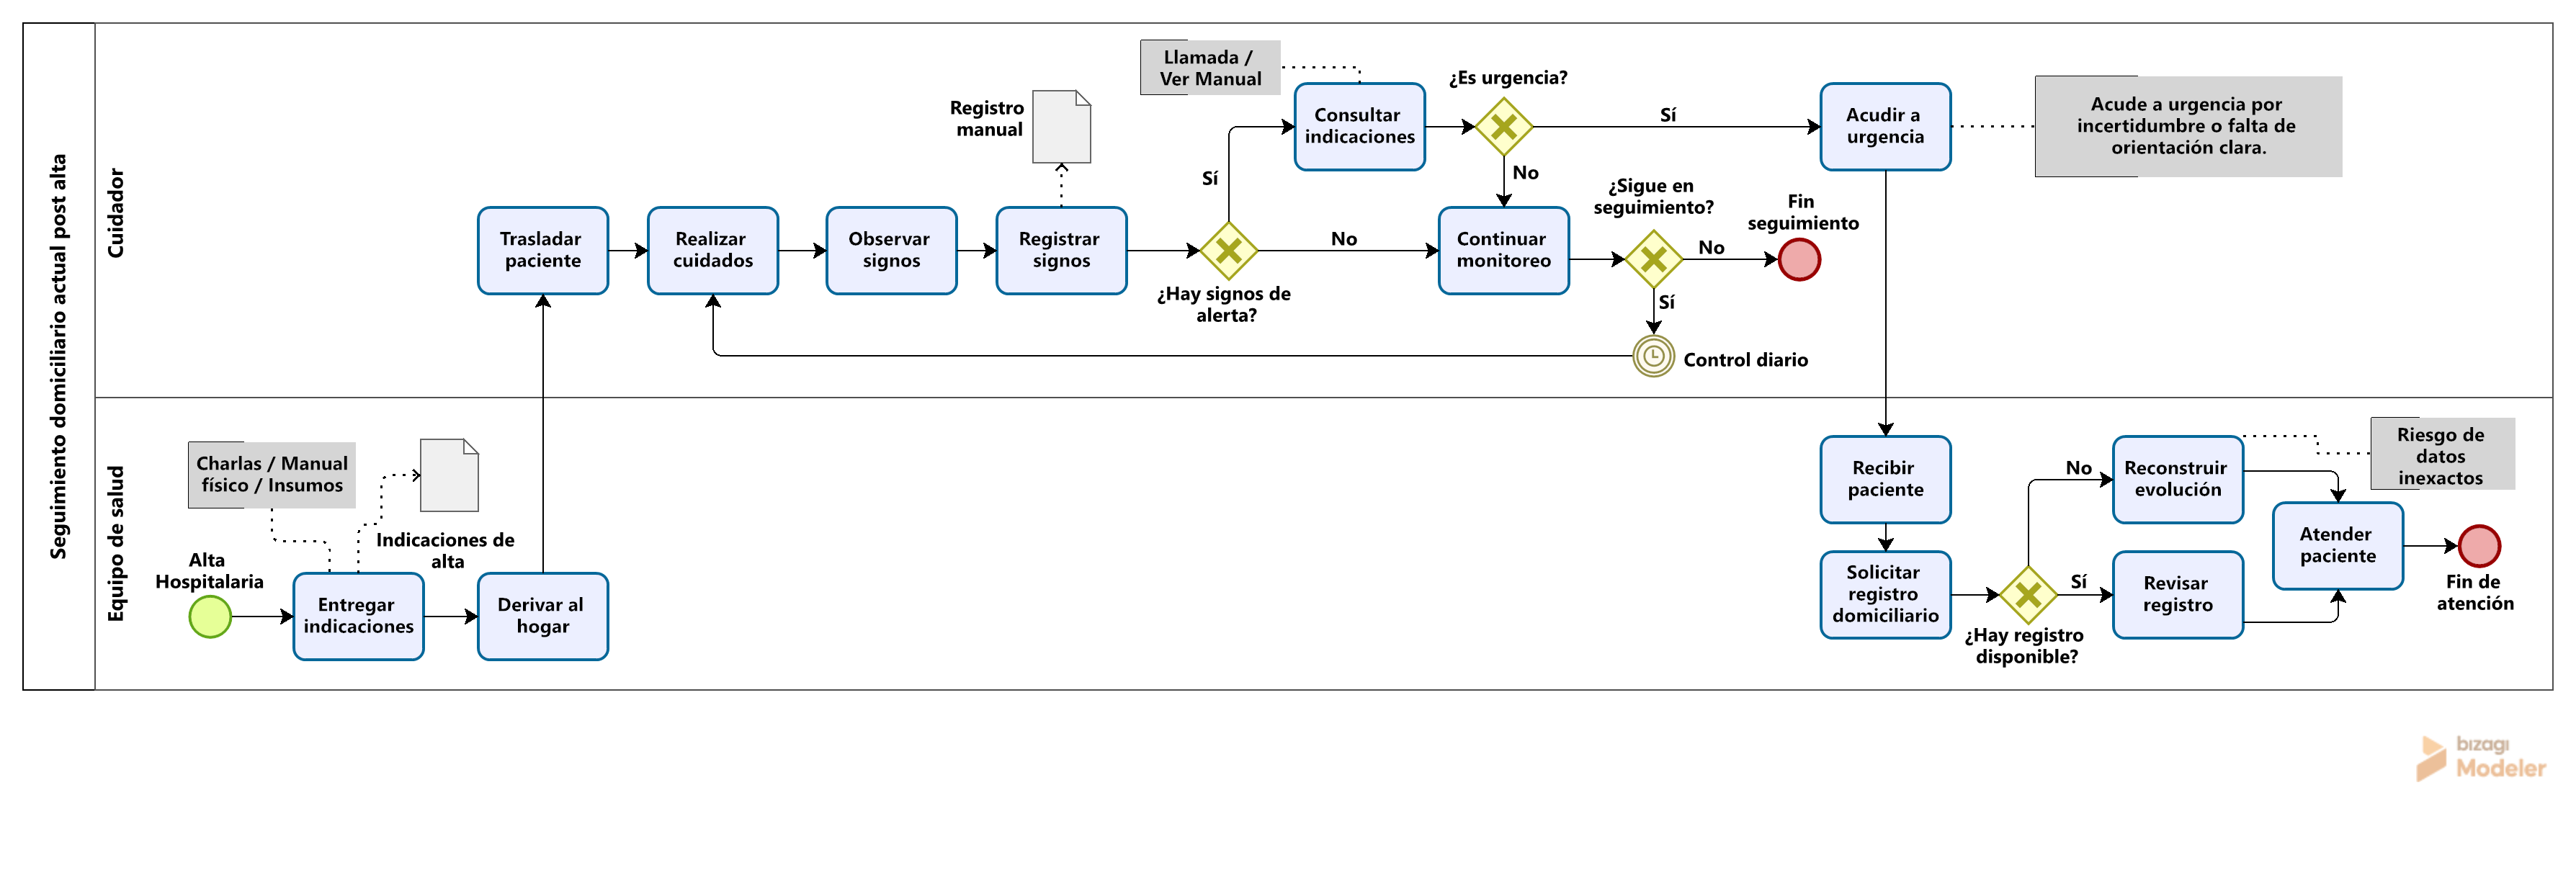
\includegraphics[width=\textwidth]{figures/proceso_negocio_actual.png}
    \caption{Proceso de negocio actual del seguimiento domiciliario.}
    \label{fig:proceso-negocio-actual}
\end{figure}

La literatura respalda la relevancia de este escenario. Los cuidadores de
pacientes oncológicos pediátricos presentan altos niveles de fatiga y sobrecarga
\citep{lewandowska_2022}, y las plataformas digitales de educación en cáncer
mejoran el conocimiento y la adherencia cuando la información está disponible en
el momento en que surge la duda \citep{nair_2017}. A su vez, el registro
estructurado de síntomas con escalas validadas como ESAS entrega al equipo
clínico antecedentes más confiables que el relato del cuidador
\citep{arnis_2024}, y los sistemas de apoyo a la decisión en el cuidado
domiciliario pediátrico favorecen la detección temprana de situaciones de riesgo
\citep{lau_2025}.

\subsection{Problemas detectados}

El problema central es la ausencia de una herramienta que apoye al cuidador en
tres tareas: registrar de forma ordenada la evolución del paciente, consultar
información educativa validada y reconocer a tiempo los signos de alerta. De él se
desprenden los siguientes problemas específicos.

\begin{enumerate}
    \item La información educativa está dispersa entre indicaciones verbales,
    manuales impresos y lo que el cuidador recuerda.
    \item Los síntomas registrados en el hogar no quedan ordenados ni disponibles
    para los controles.
    \item El cuidador no siempre distingue cuándo un síntoma requiere solo
    observación, una consulta o atención urgente.
    \item No existe un canal que resuelva dudas frecuentes con respuestas breves y
    validadas.
    \item El equipo clínico conoce la evolución entre controles solo a través de
    un relato no estandarizado.
\end{enumerate}

Estos problemas afectan a tres grupos. El cuidador vive el seguimiento con
incertidumbre y sobrecarga. El paciente queda expuesto a que un signo de alerta
se detecte tarde. El equipo clínico, por su parte, trabaja con información
domiciliaria incompleta.

De este diagnóstico nace el objetivo del sistema, que es entregar al cuidador
principal una aplicación móvil que centralice la información educativa validada,
registre de forma estructurada los signos y síntomas del paciente y lo oriente
ante signos de alerta, para dar continuidad a la atención entre el hospital y el
hogar.

\addtocontents{toc}{\protect\setcounter{tocdepth}{2}}
